\section{Blending}

The function $blending$ receives two images, the mask and the pyramid levels, it returns the blended image.

\begin{lstlisting}[language=python][h!]
blending(img_a, img_b, mask, level = 2)
\end{lstlisting}

Initially, the Laplacian pyramid of $image_a, image_b$ and Gaussian Pyramid of the $mask$ are build.

\begin{lstlisting}[language=python][h!]
lp_a = lp.laplacian_pyramid(img_a,level)
lp_b = lp.laplacian_pyramid(img_b,level)
gp_mask = gp.gaussian_pyramid(mask,level)
lp_a.build()
lp_b.build()
gp_mask.build()
\end{lstlisting}

Next, the images of each level of Laplacian pyramids are joint using its corresponding level in Gaussian pyramid of the $mask$, they are stored in $mid$.

\begin{lstlisting}[language=python][h!]
mid = []
for i in range(level - 1, -1, -1):
    mask = gp_mask.get(i)
    joint = combine(lp_a.get(i), lp_b.get(i), mask)
    mid.append(joint)
\end{lstlisting}

Finally, the same process of reconstruction as in Laplacian pyramid is done, this  yields in the blended image. As explained in the previous section, the function $down$ of the Laplacian pyramid will upsample \textit{img\_blend}(the first time \textit{img\_blend} is equivalent to the union of the last levels of Gaussian pyramids) and will sum it up with $mid[i]$, this operation is the inverse of the $up$ operation used to build the Laplacian pyramid.

\begin{lstlisting}[language=python][h!]
img_blend = mid[0]
for i in range(1, len(mid)):
	img_blend = lp_a.down(img_blend, mid[i])
return img_blend
\end{lstlisting}

The main problem during implementation was related with the size of the up sampled image and the current level: when the width or height was odd, we "lose" a row or a columns. Another problem was related with multichannel images, it is better to have a function that blends RGB or grayscale images without extra parameters or more complicated stuff, in a transparent way to the user. Thus, our implementation overcomes these problems and has not limitation in this sense, moreover there is a previous step that checks whether the size of the input images are equal such that it resize them to get valid shapes. Note that the implementation allows to set the $mask$ with left-right blending, bottom-up blending and also load a binary image as $mask$.

We performed extensive experiments with different images. The results of the blending are shown in the sub figures~\ref{fig:blending-b}, ~\ref{fig:blending-c} and ~\ref{fig:blending-d}. The blending generated by the OpenCV algorithm is shown in the sub figure~\ref{fig:blending-a}. The result of our implementation is very similar to the OpenCV one, therefore, we conclude that our implementation is going well.

\begin{figure}[h!]
\centering
\begin{subfigure}{0.33\textwidth}
  \centering
  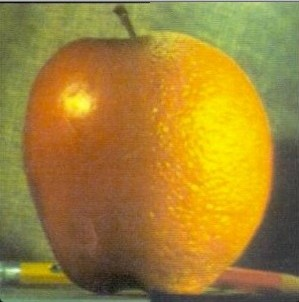
\includegraphics[width=0.8\linewidth]{output/blendedOpenCV.jpg}
  \caption{blending with \href{http://docs.opencv.org/3.1.0/dc/dff/tutorial_py_pyramids.html}{\textit{OpenCV}}.}
  \label{fig:blending-a}
\end{subfigure}%
\begin{subfigure}{0.33\textwidth}
  \centering
  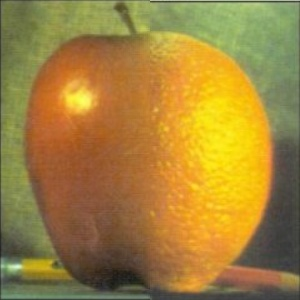
\includegraphics[width=0.8\linewidth]{output/blending1.jpg}
  \caption{Left-right blending}
  \label{fig:blending-b}
\end{subfigure}%
\begin{subfigure}{0.33\textwidth}
  \centering
  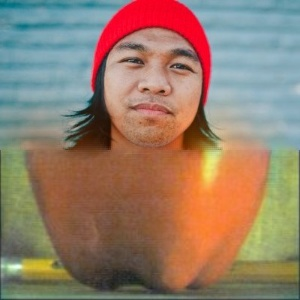
\includegraphics[width=0.8\linewidth]{output/blending2.jpg}
  \caption{Bottom-up blending}
  \label{fig:blending-c}
\end{subfigure}
\begin{subfigure}{0.7\textwidth}
  \centering
  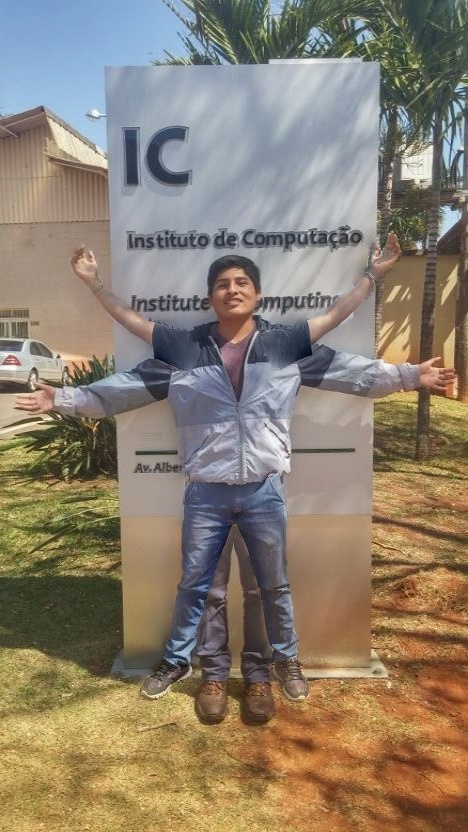
\includegraphics[width=0.8\linewidth]{output/blending.jpg}
  \caption{Binary image blending}
  \label{fig:blending-d}
\end{subfigure}%
 \caption{Blending results}
\label{fig:blending}

\end{figure}




